\documentclass[12pt, oneside]{article}

\usepackage[letterpaper, scale=0.8, centering]{geometry}
\usepackage{fancyhdr}
\setlength{\parindent}{0em}
\setlength{\parskip}{1em}

\pagestyle{fancy}
\fancyhf{}
\renewcommand{\headrulewidth}{0pt}
\rfoot{{\footnotesize Copyright Mia Minnes, 2025, Version \today~(\thepage)}}

\usepackage{titlesec}

\author{CSE105W25}

\newcommand{\instructions}{{\bf For all HW assignments:} Weekly homework 
may be done individually or in groups of up to 3 students. 
You may switch HW partners for different HW assignments. 
Please ensure your name(s) and PID(s) are clearly visible on the first page of your homework submission 
and then upload the PDF to Gradescope. If working in a group, submit only one submission per group: 
one partner uploads the submission through their Gradescope account and then adds the other group member(s) 
to the Gradescope submission by selecting their name(s) in the ``Add Group Members" dialog box. 
You will need to re-add your group member(s) every time you resubmit a new version of your assignment.
 Each homework question will be graded either for correctness (including clear and precise explanations and 
 justifications of all answers) or fair effort completeness. 
 On the ``graded for correctness"
 questions, you may only collaborate with CSE 105 students in your group; if your
 group has questions about a problem, you may ask in drop-in help hours or post a private
post (visible only to the Instructors) on Piazza. On the "graded for completeness" questions, you 
may collaborate with all other CSE 105 students this quarter, and you may make public posts about these questions 
on Piazza.

All submitted homework for this class must be typed. 
You can use a word processing editor if you like (Microsoft Word, Open Office, Notepad, Vim, Google Docs, etc.) 
but you might find it useful to take this opportunity to learn LaTeX. 
LaTeX is a markup language used widely in computer science and mathematics. 
The homework assignments are typed using LaTeX and you can use the source files 
as templates for typesetting your solutions.
To generate state diagrams of machines, you can (1) use the LaTex tikzpicture
environment (see templates in the class notes), or (2) use the software tools Flap.js or
JFLAP described in the class syllabus (and include a screenshot in your PDF), or (3) you can carefully
and clearly hand-draw
the diagram and take a picture and include it in your PDF.
We recommend that you
submit early drafts to Gradescope so that in case of any technical difficulties, at least some of your
work is present. You may update your submission as many times as you'd like up to the deadline.


{\bf Integrity reminders}
\begin{itemize}
\item Problems should be solved together, not divided up between the partners. The homework is
designed to give you practice with the main concepts and techniques of the course, 
while getting to know and learn from your classmates.
\item On the "graded for correctness"
questions, you may only collaborate with CSE 105 students in your group.
You may ask questions about the homework in office hours (of the instructor, TAs, and/or tutors) and 
on Piazza (as private notes viewable only to the Instructors).  
You \emph{cannot} use any online resources about the course content other than the class material 
from this quarter -- this is primarily to ensure that we all use consistent notation and
definitions (aligned with the textbook) and also to protect the learning experience you will have when
the `aha' moments of solving the problem authentically happen.
\item Do not share written solutions or partial solutions for homework with 
other students in the class who are not in your group. Doing so would dilute their learning 
experience and detract from their success in the class.
\end{itemize}

}

\newcommand{\gradeCorrect}{({\it Graded for correctness}) }
\newcommand{\gradeCorrectFirst}{\gradeCorrect\footnote{This means your solution 
will be evaluated not only on the correctness of your answers, but on your ability
to present your ideas clearly and logically. You should explain how you 
arrived at your conclusions, using
mathematically sound reasoning. Whether you use formal proof techniques or 
write a more informal argument
for why something is true, your answers should always be well-supported. 
Your goal should be to convince the
reader that your results and methods are sound.} }
\newcommand{\gradeComplete}{({\it Graded for completeness}) }
\newcommand{\gradeCompleteFirst}{\gradeComplete\footnote{This means you will 
get full credit so long as your submission demonstrates honest effort to 
answer the question. You will not be penalized for incorrect answers. 
To demonstrate your honest effort in answering the question, we 
expect you to include your attempt to answer *each* part of the question. 
If you get stuck with your attempt, you can still demonstrate 
your effort by explaining where you got stuck and what 
you did to try to get unstuck.} }

\usepackage{tikz}
\usetikzlibrary{automata,positioning,arrows}

\input{../../resources/discrete-math-packages}

\newcommand{\SUBSTRING}{\textsc{Substring}}
\newcommand{\REP}{\textsc{Rep}}
\newcommand{\blank}{\scalebox{1.5}{\textvisiblespace}}


\title{HW4CSE105F24: Homework assignment 4}
\date{Due: November 12, 2024 at 5pm, via Gradescope}


\begin{document}
\maketitle
\thispagestyle{fancy}

{\bf In this assignment,}

You will work with context-free languages and their representations.
You will  also practice analyzing, designing, and working with Turing machines.
You will use general constructions and specific machines to explore the classes 
of recognizable and decidable languages.


{\bf Resources}: To review the topics 
for this assignment, see the class material from Weeks 4, 5, and 6.
We will post frequently asked questions and our answers to them in a 
pinned Piazza post. 

{\bf Reading and extra practice problems}:  
Sipser Chapters 2 and 3.
Chapter 2 exercises 2.1, 2.2, 2.3, 2.4, 2.5, 2.6, 2.7, 2.9, 2.10, 2.11, 2.12, 2.13, 2.16, 2.17.
Chapter 3 exercises 3.1, 3.2, 3.5, 3.8.

\instructions

You will submit this assignment via Gradescope
(\href{https://www.gradescope.com}{https://www.gradescope.com}) 
in the assignment called ``hw4CSE105F24''.

{\bf Assigned questions}
\begin{enumerate}[wide, labelwidth=!, labelindent=0pt]

%%%%%%%%%%% PROBLEM 1 %%%%%%%%%%%
\item \textbf{Push-down automata (PDA) and context-free grammars (CFG)} (8 points): 
On page 14 of the week 3 notes, we have the following list of languages over the alphabet $\{a,b\}$

\begin{center}
\begin{tabular}{ccc}
    $\{a^nb^n \mid 0  \leq n  \leq 5 \}$
    &$\{b^n a^n \mid  n  \geq 2\}$
    &$\{a^m b^n \mid  0 \leq m\leq n\}$
\end{tabular}
\begin{tabular}{cc}
    $\{a^m b^n \mid  m \geq n+3,  n \geq 0\}$
    &$\{b^m a^n \mid  m \geq 1, n \geq  3\}$\\
    $\{ w  \in \{a,b\}^* \mid w = w^\mathcal{R} \}$
    &$\{ ww^\mathcal{R} \mid w\in \{a,b\}^* \}$ \\
\end{tabular}
\end{center}
\begin{enumerate}
    \item\gradeCompleteFirst Pick one of the regular languages and design a regular expression that describes it. 
    Briefly justify your regular expression by connecting
    the subexpressions of it to the intended language and referencing relevant definitions.
    \item\gradeComplete Pick another one of the regular languages and design a deterministic finite automaton (DFA) that recognizes it. Draw the 
    state diagram of your DFA. Briefly justify your design by explaining the role each state plays in the machine, 
    as well as a brief 
    justification about how the strings accepted and rejected by the machine connect to the specified language.
    \item\gradeComplete Pick one of the nonregular languages and design a PDA that recognizes it. Draw the state diagram of 
    your PDA. Briefly justify your design by explaining the role each state plays in the machine, 
    as well as a brief 
    justification about how the strings accepted and rejected by the machine connect to the specified language.
    \item\gradeComplete Pick one of the nonregular languages and write a CFG that generates it. Briefly justify
    your design by by demonstrating how derivations in the grammar relate
    to the intended language.
\end{enumerate}

%%%%%%%%%%% PROBLEM 2 %%%%%%%%%%%
\item \textbf{General constructions for context-free languages} (21 points):

In class in weeks 4 and 5, we described several general constructions 
with PDAs and CFGs, leaving their details to
homework. In this question, we'll fill in these details. The first constructions
help us prove that the class of regular languages is a subset of the
class of context-free languages. The other construction allows us 
to make simplifying assumptions about PDAs recognizing languages.

\begin{enumerate}

\item\gradeCorrectFirst When we first introduced PDAs we observed 
that any NFA can be transformed to a PDA by not using the stack 
of the PDA at all. Suppose a friend gives you the following construction
to formalize this transformation:

\begin{quote}
Given a NFA $N = (Q, \Sigma, \delta_N, q_0, F)$ we define a PDA $M$
with $L(M) = L(N)$ by letting $M = ( Q, \Sigma, \Sigma, \delta, q_0, F)$ where 
$\delta(~(q,a,b)~) = \delta_N(~(q,a)~)$ for each $q \in Q$, 
$a \in \Sigma_{\varepsilon}$ and $b \in \Sigma_{\varepsilon}$.
\end{quote}

For each of the six defining parameters for the PDA, explain whether 
it's defined correctly or not. If it is not defined correctly, 
explain why not and give a new definition for this parameter that 
corrects the mistake.

\item\gradeCorrect In the book on page 107, the top paragraph describes a procedure for converting DFAs to CFGs:
\begin{quote}
   You can convert any DFA into an equivalent CFG as follows. 
   Make a variable $R_i$ for each state $q_i$ of the DFA. Add the rule $R_i \to aR_j$ to the
   CFG if $\delta(q_i,a) =q_j$ is a transition in the DFA. Add the rule
   $R_i\to \varepsilon$ if $q_i$ is an accept state of the DFA. Make $R_0$ the start variable ofthe grammar, 
   where $q_0$ is the start state of the machine. Verify on your own that the resulting CFG 
   generates the same language that the DFA recognizes.
\end{quote}

Use this construction to get a context-free grammar generating the language 
\[
    \{ w \in \{0,1\}^* \mid w \text{ does not end in  $101$}\}
\]
by (1) designing a DFA that recognizes this language and then (2) applying the construction from the book to convert the 
DFA to an equivalent CFG. A complete and correct submission will include the state diagram of the DFA, a brief justification of why 
it recognizes the language, and then the complete and precise definition of the CFG that results from applying the construction 
from the book to this DFA. {\it Ungraded bonus: take a sample string in the language and see how the computation of 
the DFA on this string translates to a derivation in your grammar.}

\item Let $M_1 = (Q_1, \Sigma, \Gamma_1, \delta_1, q_1, F_1)$ 
be a PDA and let $q_{new}, r_{new}, s_{new}$ be three fresh state labels 
(i.e. $Q_1 \cap \{q_{new}, r_{new}, s_{new}\} = \emptyset$) 
and let $\#$ be a fresh stack symbol (i.e. $\# \notin \Gamma_1$).
We define the PDA $M_2$ as
\[
   (Q_2, \Sigma, \Gamma_2, \delta_2, q_{new}, \{s_{new}\})
\]
with $Q_2 = Q_1 \cup \{q_{new}, r_{new}, s_{new}\}$ 
and $\Gamma_2 = \Gamma_1 \cup \{\#\}$
and 
$\delta_2 : Q_2 \times \Sigma_\varepsilon \times {\Gamma_2}_\varepsilon \to 
\mathcal{P}(Q_2 \times {\Gamma_2}_\varepsilon)$ given by 
\[
\delta_2 ( ~(q,a,b)~) = 
\begin{cases}
\{(q_1, \#)\} &\text{if } q = q_{new}, a = \varepsilon, b = \varepsilon\\
\delta_1( ~(q,a,b)~) &\text{if } q\in Q_1 \setminus F_1, a \in \Sigma_{\varepsilon}, b \in {\Gamma_1}_\varepsilon \\
\delta_1( ~(q,a,b)~) &\text{if } q\in F_1, a \in \Sigma, b \in {\Gamma_1}_\varepsilon \\
\delta_1( ~(q,a,b)~) &\text{if } q\in F_1, a =\varepsilon, b \in {\Gamma_1} \\
\delta_1( ~(q,a,b)~) \cup \{(r_{new}, \varepsilon)\} &\text{if } q\in F_1, a =\varepsilon, b =\varepsilon \\
\{(r_{new}, \varepsilon)\} &\text{if } q = r_{new}, a =\varepsilon, b \in \Gamma_{1} \\
\{(s_{new}, \varepsilon)\} &\text{if } q= r_{new}, a = \varepsilon, b = \#\\
\emptyset & \text{otherwise}
\end{cases}
\]
for each $q \in Q_2$, $a \in \Sigma_{\varepsilon}$, 
and $b \in {\Gamma_2}_\varepsilon$.

In this question, we'll apply this construction for a specific PDA and 
use this example to extrapolate the effect of this construction.
\begin{enumerate}

\item\gradeCorrect Consider the PDA $M_1$ with input alphabet $\{0,1\}$ 
and stack alphabet $\{0,1\}$ whose state diagram is

\begin{center}

   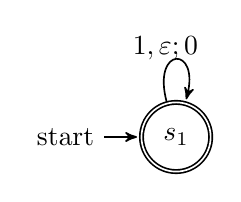
\begin{tikzpicture}[->,>=stealth',shorten >=1pt, auto, node distance=2cm, semithick]
      \tikzstyle{every state}=[text=black, fill=none]
    
    \node[initial,state, accepting] (s1)          {$s_1$};

    \path (s1) edge  [loop above, near start] node {$1,\varepsilon; 0$} (s1)
    ;
    \end{tikzpicture}
\end{center}

Draw the state diagram for the PDA $M_2$ that results from applying 
the construction to $M_1$.

\item\gradeComplete Compare $L(M_1)$ and $L(M_2)$. Are these sets 
equal? Does your answer depend on the specific choice of $M_1$? Why or why not?

\item\gradeComplete Consider the PDA $N$ with input alphabet $\{0,1\}$ and
stack alphabet $\{0,1\}$ whose state diagram is 

\begin{center}
   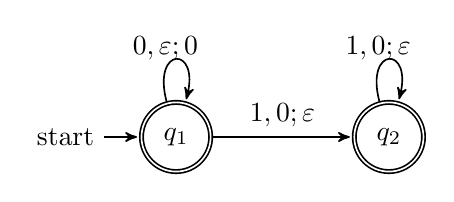
\begin{tikzpicture}[->,>=stealth',shorten >=1pt, auto, node distance=2cm, semithick]
      \tikzstyle{every state}=[text=black, fill=none]
    
    \node[initial,state, accepting] (q1)          {$q_1$};
    \node[state, accepting]         (q2) [right of=q1, xshift=20pt] {$q_2$};
    
    \path (q1) edge  [loop above, near start] node {$0,\varepsilon; 0$} (q1)
        (q1) edge [bend left=0] node {$1,0;\varepsilon$} (q2)
        (q2) edge [loop above, near start] node {$1,0;\varepsilon$} (q2)
    ;
    \end{tikzpicture}

\end{center}

   Remember that the definition of set-wise concatenation is:
    for languages $L_1, L_2$ over the alphabet $\Sigma$, we have the 
    associated set of strings
    \[
       L_1 \circ L_2 = \{ w \in \Sigma^* ~|~ w = uv \text{ for some strings } u \in L_1 \text{ and } v \in L_2 \}
    \]
    In class, we discussed how extrapolating the construction that we used to prove that the class of regular languages
    is closed under set-wise concategation by drawing 
    spontaneous transitions from the accepting states in the first 
    machine to the start state of the second machine doesn't work.
    Use the example of $M_1$ and $N_1$ to prove this by showing that
    \[
    L(M_1) \circ L(N)
    \]
    is {\bf not} the language recognized by the machine 
    results from taking the two machines
    $M_1$ and $N$, setting the start state of $M_1$ to be the start state of 
    the new machine, setting the set of accepting states of $N$ to be
    the set of accepting states of the new machine, and drawing spontaneous 
    arrows from the accepting states
    of $M_1$ to the start state of $N$.

    \item\gradeComplete Describe the language recognized by the machine 
    that results from taking the two machines
    $M_2$ and $N$, setting the start state of $M_2$ to be the start state of 
    the new machine, setting the set of accepting states of $N$ to be
    the set of accepting states of the new machine, and drawing spontaneous 
    arrows from the accepting states
    of $M_2$ to the start state of $N$. Use this description 
    to explain why we used the construction of $M_2$ from $M_1$
    and how this construction could be used in a proof of the 
    closure of the class of context-free languages under set-wise concatenation.
\end{enumerate}

\end{enumerate}
%%%%%%%%%%% PROBLEM 3 %%%%%%%%%%%
\item \textbf{Turing machines} (12 points):

Consider the Turing machine $T$ over the input alphabet $\Sigma = \{0,1\}$ with  the state
    diagram below (the tape alphabet is $\Gamma = \{ 0,1,X,\square\}$).  
    Convention: we do not include the node for the reject state $qrej$ and any missing transitions in the state diagram have value $(qrej,\square,R)$
    \begin{center}
      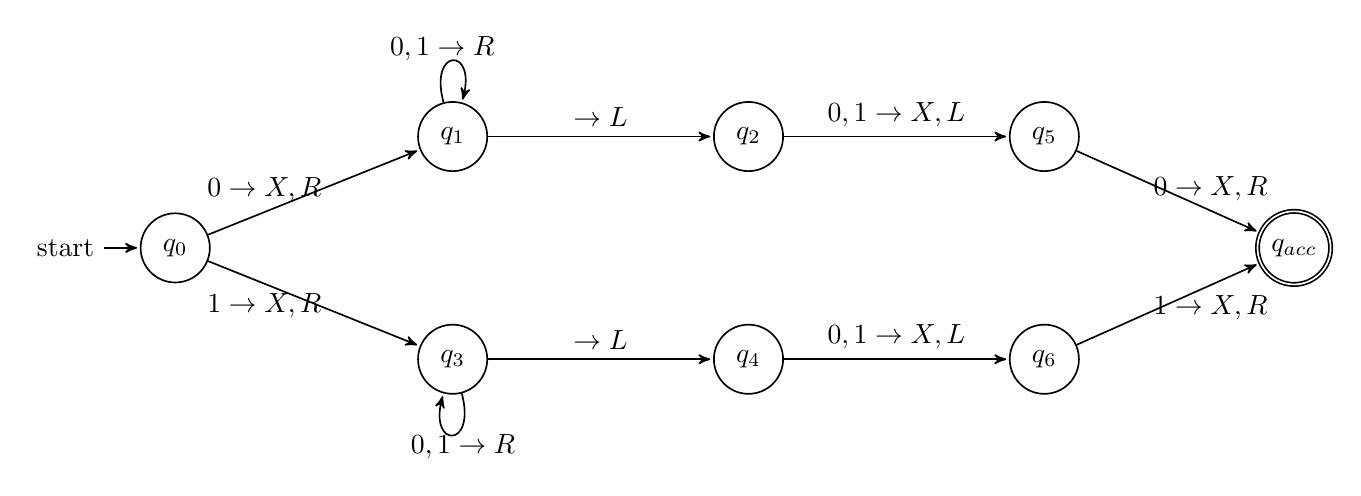
\begin{tikzpicture}[->,>=stealth',shorten >=1pt, auto, node distance=2cm, semithick]
         \tikzstyle{every state}=[text=black, fill=none]
        
        \node[initial,state] (q0)          {$q_0$};
        \node[state] (q1)  [above right of=q0, xshift=60pt] {$q_{1}$};
        \node[state] (q2)  [right of=q1, xshift=50pt] {$q_{2}$};
        \node[state] (q3)  [below right of=q0, xshift=60pt] {$q_{3}$};
        \node[state] (q4)  [right of=q3, xshift=50pt] {$q_{4}$};
        \node[state] (q5)  [right of=q2, xshift=50pt] {$q_5$};
        \node[state] (q6)  [right of=q4, xshift=50pt] {$q_6$};
        \node[state, accepting]         (qacc) [below right of=q5, xshift=50pt] {$q_{acc}$};
        
        \path (q1) edge  [loop above, near start] node {$0,1 \to R$} (q1)
            (q3) edge  [loop below, near start] node {$0,1 \to R$} (q3)
            (q0) edge [bend left=0, above, near start] node {$0\to X, R$} (q1)
            (q0) edge [bend left=0, below, near start] node {$1\to X, R$} (q3)
            (q1) edge [bend left=0] node {$\square \to L$} (q2)
            (q3) edge [bend left=0] node {$\square \to L$} (q4)
            (q2) edge [bend left=0] node {$0,1 \to X, L$} (q5)
            (q4) edge [bend left=0] node {$0,1 \to X, L$} (q6)
            (q5) edge [bend left=0, above, near end] node {$0\to X, R$} (qacc)
            (q6) edge [bend left=0, below, near end] node {$1\to X, R$} (qacc)
        ;
        \end{tikzpicture}
    \end{center}

    \begin{enumerate}

        \item\gradeCorrect Specify an example string $w_1$ of length $4$ over 
        $\Sigma$ that is {\bf accepted} by this Turing machine, or explain why there is no such 
        example. A complete solution will include either (1) a precise and clear 
        description of your example  string and a precise and clear description of the accepting computation
        of the Turing machine on this string or (2) a sufficiently
        general and correct argument why there is no such example, referring back to the relevant definitions.
        
        To describe a computation of a Turing machine, include the contents of the 
        tape, the state of the machine, and the location of the read/write head at each step in the computation.
        
        {\it Hint:} In class we've drawn pictures to represent the configuration of the machine at each step 
        in a computation.  You may do so or you may choose to describe these configurations in words.
        
        \item\gradeCorrect Specify an example string $w_2$ of length $3$ over $\Sigma$ 
        that is {\bf rejected} by this Turing machine
        or explain why there is no such 
        example. A complete solution will include either (1) a precise and clear 
        description of your example  string and a precise and clear description of the rejecting computation
        of the Turing machine on this string or (2) a sufficiently
        general and correct argument why there is no such example, referring back to the relevant definitions.

        \item\gradeCorrect Specify an example string $w_3$ of length $2$ over $\Sigma$ 
        on which  the computation of this Turing machine is {\bf never halts}
        or explain why there is no such 
        example. A complete solution will include either (1) a precise and clear 
        description of your example  string and a precise and clear description of the looping (non-halting) 
        computation
        of the Turing machine on this string or (2) a sufficiently
        general and correct argument why there is no such example, referring back to the relevant definitions.

        {\it Note}: when a Turing machine does not halt on a given input string, 
        we say that it {\bf loops} on that string.

\end{enumerate}



%%%%%%%%%%% PROBLEM 4 %%%%%%%%%%%
\item\textbf{Implementation-level descriptions of deciders and recognizers} (9 points):

For this question, consider the alphabet $\Sigma = \{a,b,c\}$.
\begin{enumerate}
\item[(a)]\gradeCorrect Give an example of an infinite language over $\Sigma$ (that is not $\Sigma^*$) and give
two different Turing machines that recognize it: one that is a decider and one that is not.
A complete solution will include a precise definition for your example language, 
along with {\bf both} a state diagram and an implementation-level description 
of each Turing machines, along with a brief explanation of why each of them recognizes
the language and why one is a decider and there other is not.

\item[(b)]\gradeComplete True or false: There is a Turing machine that is not a decider that recognizes 
the empty set. A complete solution will include a witness Turing machine (given by 
state diagram or implementation-level description or high-level description) and a justification 
for why it's not a decider and why it does not accept any strings, or a complete and correct
justification for why there is no such Turing machine.

\item[(c)]\gradeComplete True or false: There is a Turing machine that is not a decider that recognizes 
the set of all string $\Sigma^*$.  A complete solution will include a witness Turing machine 
(given by 
state diagram or implementation-level description or high-level description) and a justification 
for why it's not a decider and why it accept each string over $\{a,b,c\}$, or a complete and correct
justification for why there is no such Turing machine.
\end{enumerate}
\end{enumerate}
\end{document}